\section{Evaluation}
First and foremost, we might want to consider the difference in performace of
our two approaches. \textbf{T5-finetuned} and \textbf{T5-finetuned\(^2\)}. This
will help us identify whether the additional training is beneficial for the
task.

\begin{minipage}{\linewidth}
    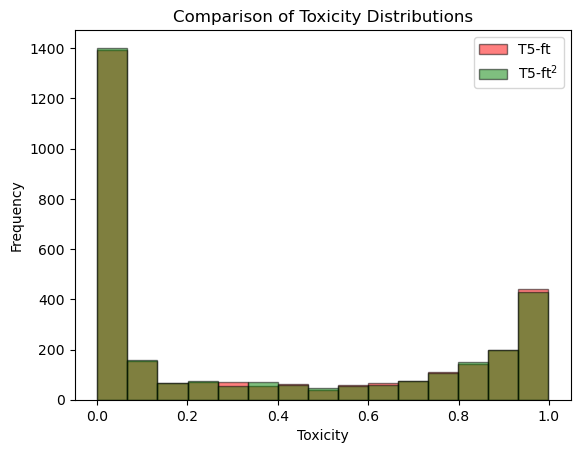
\includegraphics[scale=0.35]{figures/final/t5-52-toxicity.png}% 
    \figcaption{Toxicity distribution}% 
    \label{fig:eval:toxdistrt52}% 
\end{minipage}

\begin{minipage}{0.9\linewidth}
    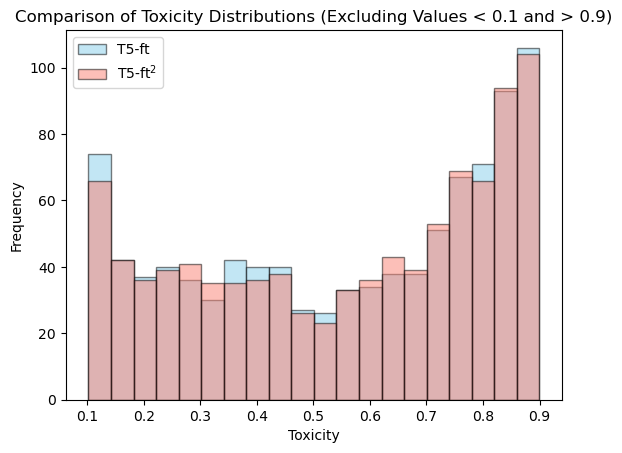
\includegraphics[scale=0.35]{figures/final/t5-52-tox-limited.png}% 
    \figcaption{Toxicity distribution (limited)}% 
    \label{fig:eval:toxdistrlimt52}% 
\end{minipage}

\end{multicols*}
\begin{minipage}{\linewidth}
    \centering% 
    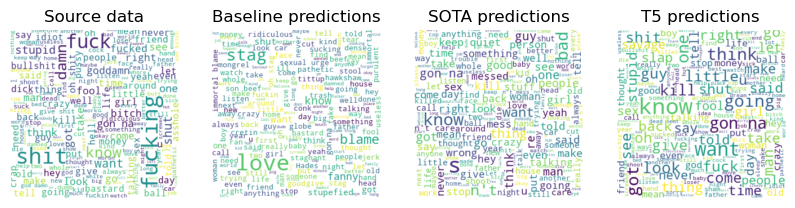
\includegraphics[scale=0.6]{figures/final/wordcloud.png}% 
    \figcaption{Wordclouds comparison}% 
    \label{fig:eval:wordcloud}% 
\end{minipage}
\begin{multicols*}{2}

As we can derive from the toxicity distributions, models are practically
identical and no any significant improvement in performance was introduced.
Moreover, additional training added more computational and time overhead. As a
result, we might want to further consider only the first approach, without
additional training.

We can conclude, that the issue with the \textbf{T5} model as base is not in
it's fine-tuning, rather than the capabilities of the model itself. Extending
the tuning dataset will not improve it's capabilities and other approach in
future is required.

Further on, we can consider first the wordcloud of the corresponding models. We
can see that the source data has a lot of swear words, which are very frequent.
Wordcloud is quite good representation for this type of data.

If we consider \textbf{baseline} predictions on the very same figure, we can
see that predictions are not perfect either. While the word ``love'' is
considered the most frequent, on the second place there is ``stag'', which is,
most probably, used in a toxic context. Moreover, we can find a lot of
evidently swear words in the cloud.

Completely the other side of a coin represents the \textbf{SOTA} approach. It
is difficult to find swear word in the cloud, even if any of them are there.
This is a very good result, as it completely removed the open toxicity.

Somewhat in the middle is the \textbf{T5-finetuned} approach. While it
generally has great results and cloud lacks such dense distribution of bad
words, it did not eliminate all of them. At least they are not so densely
populated as in the baseline solution.

\begin{minipage}{\linewidth}
    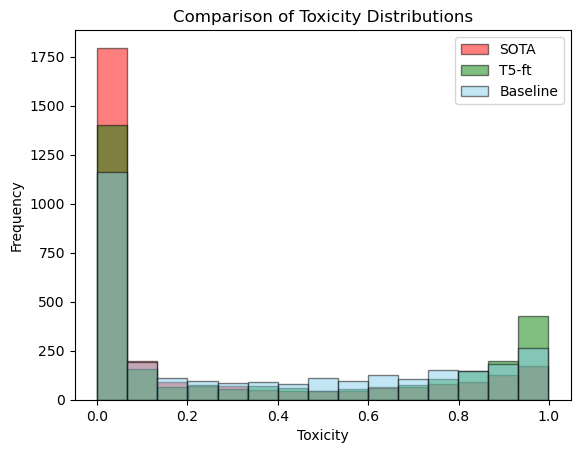
\includegraphics[scale=0.35]{figures/final/toxicity.png}% 
    \figcaption{Toxicity distribution}% 
    \label{fig:eval:toxdistr}% 
\end{minipage}

\subsection{Toxicity}

We can analyze the toxicity distribution of all three models and consider the
reasons of such differences. First of all, we can notice that toxicity
distribution is approximately the same. It means that the sentences the models
struggle most are most probable relatively the same. Some of models just
perform a bit better and some of them a bit worse.

Evidently, \textbf{SOTA} technique has the best score in the distribution close
to zero, meaning it is the best approach to clean up the sentences. As well as
the \textbf{T5-finetuned} is the second place. However, we can see that
\textbf{T5-finetuned} struggles the most on difficult sentences, as the number
of sentences with toxicity close to one is the largest. Most probably, baseline
solution is better in right most distribution because is better at detecting
the bad words in senteces, but not necessarily better at preserving the
meaning. The reason for this, baseline simply matches the swear words, while
\textbf{T5-finetuned} can be easilly fooled by difficult and confusing
formulations.

\begin{minipage}{0.9\linewidth}
    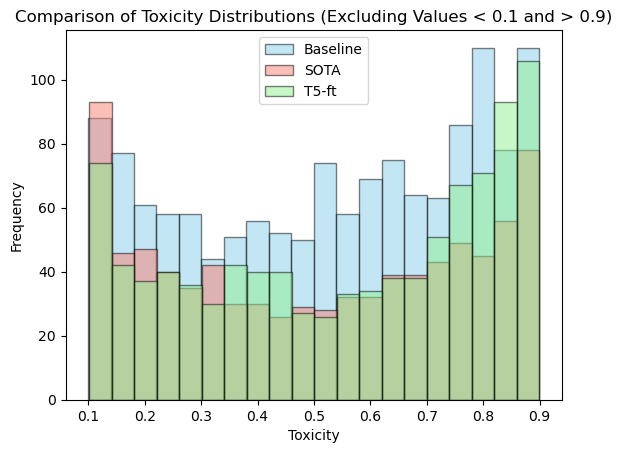
\includegraphics[scale=0.35]{figures/final/toxicity-limited.png}% 
    \figcaption{Toxicity distribution (limited)}% 
    \label{fig:eval:toxdistrlim}% 
\end{minipage}

A bit better representation of the distribution can be seen on the
figure~\ref{fig:eval:toxdistrlim}. Limiting the \(x\) axis of the figure for
edge cases, we can see comparison of average models performance on the data.

Surprisingly, we can see, that \textbf{T5-finetuned} and \textbf{SOTA} have
pretty similar distributions just like they were same models with slightly
different effectiveness. However, \textbf{baseline} is definitely just bad in
this case. On a larger test set this difference could have been even larger.

\subsection{Semantic similarity}

\begin{minipage}{\linewidth}
    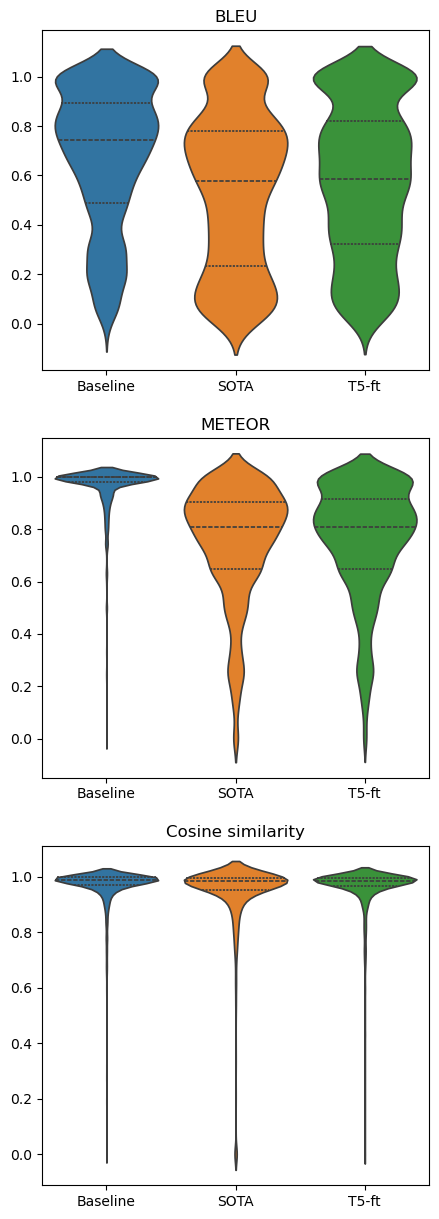
\includegraphics[scale=0.4]{figures/final/semantic.png}% 
    \figcaption{Semantic comparison}% 
    \label{fig:eval:toxdistrlim}% 
\end{minipage}

Analysis of semantic similarities between the source and prediction can lead to
interesting results as well. For this we will use violin plots, representing
the distribution of the certain value in the dataset. Finally, we will add
lines, denoting quartiles of the data distribution, as it will become useful in
the future.

For instance, very expected result is the victory of \textbf{baseline} model
over all other metrics. The key to success is the cherrypicking of the word it
replaces, leaving everything as it was before. As a result, overall score
becomes incredibly large, since the sentences practically identical. Even
unsuitable synonyms can not affect the overall result of the model. However, as
we saw previously, this result comes at cost of the worst detoxification
results and meaning violation.

More interesting conclusions we can make comparing the \textbf{T5-finetuned}
with the \textbf{SOTA} algorithm. The overall patterns of the result again
confirm the suspicious similarity of the models. Overall shape of the
distribution, as well as quartiles generally reflect the same shapes of
predictions.

Moreover, \textbf{T5-finetuned} tends to have slightly better semantic scores
than the \textbf{SOTA} model. The reason for this is the preservation of the
overall structure of the sentence. While being seemingly built around the
similar model, \textbf{SOTA} is slightly better at paraphrasing, such as
``dickheads'' becomes ``bad guys''.

Therefore, every metric comes at a cost. \textbf{T5-finetuned} is better at
preserving the initial structure of the sentence, but worse in detoxification.
Conversely \textbf{SOTA} approach is better at detoxification, due to
non-preservation of initial structure.